\documentclass[sigconf,natbib=true,anonymous]{acmart}
%% RecSys 2026 — Main Track Long Paper (8 pages content + unlimited references)
%% Uses ACM sigconf format (two-column layout), double-blind review.
%% Camera-ready: remove 'anonymous' and add author info.

%% Remove ACM-specific elements for cleaner review copy
\settopmatter{printacmref=false}
\renewcommand\footnotetextcopyrightpermission[1]{}
\setcopyright{none}
\acmConference[RecSys'26]{Proceedings of the 20th ACM Conference on Recommender Systems}{September 2026}{TBD}
\acmYear{2026}
\acmDOI{}
\acmISBN{}

\usepackage{booktabs}
\usepackage{multirow}
\usepackage{amsmath,amssymb}
\usepackage{algorithm}
\usepackage{algpseudocode}
\usepackage{graphicx}
\usepackage{subcaption}
\usepackage{siunitx}
\usepackage{xspace}
\usepackage{enumitem}
\usepackage{microtype}
\usepackage{ifthen}
\usepackage{balance}  % Balance columns on last page
\usepackage{hyperref} % Required for \url{} in abstract & body

\newcommand{\model}{\textsc{MV-Align}\xspace}
\newcommand{\base}{\textsc{SASRec}\xspace}
\newcommand{\tfidf}{\textsc{TF-IDF}\xspace}
\newcommand{\llm}{\textsc{LLM}\xspace}
\newcommand{\InfoNCE}{InfoNCE\xspace}

% Circled numbers for figure captions (using textcomp to avoid tikz/amssymb conflict)
\usepackage{pifont}
\newcommand*\circled[1]{\ding{\numexpr171+#1\relax}}

\begin{document}

\title{MV-Align: Multi-View Text Alignment with Explicit Feature Crossing\\
for Sequential Recommendation}

% Review version: anonymous authors.
% Camera-ready example:
% \author{First Author}
% \affiliation{\institution{Institution}\country{Country}}
% \email{email@example.com}

\begin{abstract}
Incorporating text features into sequential recommenders can substantially improve generalization, especially for cold-start items, yet prior methods typically rely on a single text representation and fuse it with ID embeddings only implicitly through shared attention layers.
We argue that this design misses two opportunities: (i)~diverse prompt-driven \llm views capture complementary item semantics that a single embedding cannot, and (ii)~explicit feature crossing between ID and text signals---well established in CTR prediction but unexplored in sequential recommendation---can sharpen ranking quality.
%
We propose \model, which introduces three novel components on top of a \base backbone: \emph{per-view whitening} that decorrelates multi-view \llm embeddings before fusion, \emph{explicit ID$\times$Text cross interactions} via DCN-V2, and \emph{multi-view contrastive alignment} with cold-start reweighting.
Through controlled ablations under full-ranking evaluation on Amazon Beauty and Toys\&Games, we expose a previously unreported \textbf{HR--ranking trade-off}: enabling the cross network improves ranking precision (MRR/NDCG) at the cost of recall (HR), while disabling it reverses this balance---a finding that directly maps to deployment choices between candidate generation and final re-ranking.
%
\model achieves HR@10 of \textbf{5.79}\% and \textbf{6.61}\% (+6.8\% and +11.7\% over ID-only), and under equal embedding bandwidth, multi-view prompting narrows the cold-start HR\_new gap to ID-only on Beauty (1.76\% vs.\ 1.88\%) while exceeding it on Toys (2.04\% vs.\ 1.92\%), achieving the best cold-start ranking quality (NDCG\_new and MRR\_new) on both datasets.
Code and configurations are available at \texttt{\url{https://anonymous.4open.science/r/recbole-multiview-D83A}}.
\end{abstract}

\keywords{Sequential Recommendation, Text-Enhanced Recommendation, Multi-View Representation, Feature Crossing, Contrastive Alignment, Cold-Start}

\maketitle

\section{Introduction}

Modern sequential recommenders such as \base~\cite{kang2018sasrec}
provide a strong backbone for modeling user behavior sequences,
yet real-world catalogs are dominated by cold-start and long-tail
items where collaborative signals are sparse. Item text (titles,
descriptions, reviews) offers semantic cues that can improve
generalization, but it also introduces an operational tension:
lightweight features (e.g., \tfidf) are cheap and surprisingly
strong, while \llm-derived embeddings can be richer yet
substantially more expensive in extraction, storage, and serving.

A natural question is whether multi-view \llm features justify
the added complexity. We quantify this by reporting trainable
parameters and forward-pass FLOPs (Table~\ref{tab:params}) and
analyzing offline encoding cost in \S\ref{sec:complexity}.

Two practical observations motivate this work. First, once a
strong \tfidf baseline is in place (e.g., +2.6\% HR@10 and
+25.9\% NDCG@10 on Beauty under full ranking), the marginal
gains from adding \llm features can be small and domain-dependent,
making it unclear when multi-view prompting is worth the extra
offline encoding and modest incremental trainable overhead
(\S\ref{sec:experiments}). Second, model selection in industry often relies on fast
sampled evaluation (uniform-100 negatives), but
sampled metrics can disagree with full-ranking metrics and even
mis-rank models~\cite{krichene2020sampledmetrics}; this mismatch
is particularly harmful when improvements concentrate on
cold-start/long-tail strata.

\model addresses this contradiction with a simple
``prepare--interact--align'' recipe (Figure~\ref{fig:framework}):

\textbf{(1) Prepare} (representation level): We normalize
and whiten each text view independently to address three failure
modes---scale mismatch across views, view-to-view correlation,
and cross-view redundancy. Whitening decorrelates multi-view
channels, making subsequent interactions more learnable.

\textbf{(2) Interact} (fusion level): We use an explicit cross
network (DCN-V2) to learn high-order ID$\times$text feature
crosses. While Transformer self-attention models sequence-level
item--item dependencies, it does not explicitly capture
feature-level interactions between ID embeddings and text
embeddings; DCN-V2 fills this gap through element-wise products
gated by learned weight matrices.

\textbf{(3) Align} (objective level): We align each text view
to the collaborative ID embedding space via InfoNCE contrastive
loss. Alignment targets are (text view $\to$ ID space); positive
pairs are (item's text view, item's ID embedding); negatives are
in-batch items. Cold-start reweighting prevents frequent items
from dominating the alignment signal, ensuring that
low-popularity items receive sufficient gradient updates.

Our contributions are threefold.
\begin{itemize}[leftmargin=*,itemsep=1pt]
  \item \textbf{Systematic method design.} We propose \model, a
    principled framework that combines explicit cross networks (DCN-V2)
    with multi-view \llm text features for sequential recommendation.
    The ``prepare--interact--align'' design jointly leverages per-view
    whitening, explicit ID$\times$Text crossing, and contrastive
    alignment with cold-start reweighting---a combination that, to our
    knowledge, has not been explored in this setting.
  \item \textbf{New empirical finding.} Through controlled ablations
    under full-ranking evaluation on two Amazon domains with
    popularity-stratified analysis, we expose a previously unreported
    \textbf{HR--ranking trade-off}: the cross network sharpens ranking
    quality (MRR/NDCG) at the cost of recall (HR), providing
    actionable guidance for practitioners choosing between candidate
    generation and final re-ranking configurations.
  \item \textbf{Practical design insights.} We show that lightweight
    \tfidf alone is a surprisingly strong baseline, and that under
    equal embedding bandwidth ($4{\times}64$-d vs.\ $1{\times}256$-d),
    multi-view prompting consistently outperforms single-view,
    with the largest gains on cold-start items.
\end{itemize}
We organize our study around four research questions:
\textbf{RQ1}~Does per-view whitening improve text feature quality?
\textbf{RQ2}~Does SE-style channel gating help?
\textbf{RQ3}~Under equal embedding bandwidth, does multi-view outperform single-view?
\textbf{RQ4}~What are the individual contributions of explicit cross and contrastive alignment?
The rest of the paper is organized as follows: we review
related work, introduce \model, present full-ranking results
and ablations, and conclude with analyses and takeaways.

%% [Figure 1 (cover/teaser) removed per advisor feedback — overlaps with Figure 2.
%%  Retained in anonymous repo for poster / presentation use.]

\section{Related Work}
\paragraph{Sequential recommendation.}
Transformer-based sequential models such as
\base~\cite{kang2018sasrec} and BERT4Rec~\cite{sun2019bert4rec}
(which adopts bidirectional masked prediction) are strong backbones for
capturing user behavior patterns.
GRU4Rec~\cite{hidasi2016gru4rec} pioneered RNN-based session
modeling, while SASRec introduced self-attention for next-item
prediction with causal masking. Recent efficient variants
include LightSANs~\cite{fan2021lightsans} with low-rank
attention decomposition for reduced complexity.

\paragraph{Text-enhanced recommendation.}
\begin{sloppypar}
Item text features (from bag-of-words, neural encoders, or
\llm embeddings) provide complementary signals beyond
collaborative filtering. Early work used TF-IDF and
Item2Vec~\cite{barkan2016item2vec} for item representation;
CDL~\cite{wang2015cdl} jointly modeled text via stacked
denoising autoencoders. Recent approaches leverage pretrained
language models: UniSRec~\cite{hou2022unisrec} uses
BERT-encoded item text as universal transferable
representations, while VQ-Rec~\cite{hou2023vqrec} bridges
language and collaborative semantics via vector quantization.
Large language models have further expanded this line:
P5~\cite{geng2022p5} unifies recommendation in a text-to-text
paradigm, and TALLRec~\cite{bao2023tallrec} aligns LLMs with
recommendation via instruction tuning.
However, these methods typically encode item text with a single
prompt or representation.
Our work explores \emph{multi-view} \llm embeddings via diverse
prompt perspectives (identity, function, audience, and category),
with explicit fusion and alignment, and we show when this added
complexity is justified versus simpler alternatives.
\end{sloppypar}

\paragraph{Feature interaction and cross networks.}
Deep \& Cross Network (DCN)~\cite{wang2017dcn} and its
successor DCN-V2~\cite{wang2021dcnv2} explicitly model feature
crosses, complementing implicit interactions learned by DNNs.
Squeeze-and-Excitation Networks (SENet)~\cite{hu2018senet}
introduced channel-wise attention for adaptive feature
recalibration; FiBiNET~\cite{huang2019fibinet} adapted SENet
for CTR prediction with bilinear feature interactions. In
recommendation, cross networks have shown effectiveness in CTR
prediction; we adapt them for ID-text fusion in sequential
settings, and use SE-style blocks for per-view channel gating of \llm
features.

\paragraph{Multi-view learning in recommendation.}
Multi-view learning leverages complementary information from
different feature sources or modalities. Inspired by
CLIP~\cite{radford2021clip}, which aligns visual and textual
representations via contrastive learning, we design multi-view
prompts to elicit diverse semantics from language models. In
recommendation, multi-view graph neural approaches have been explored for
session-based settings~\cite{huang2025mvcgnn_session}. Our work applies
multi-view learning to \llm text embeddings, using different
prompt perspectives (identity, function, audience, category)
and whitening to decorrelate view representations before
fusion.

\paragraph{Contrastive learning in recommendation.}
Contrastive objectives such as \InfoNCE~\cite{oord2018cpc}
have been widely adopted for self-supervised representation
learning. In recommendation, contrastive methods align
user/item representations across views~\cite{wu2021cl4rec}.
We extend this to multi-view text-to-ID alignment with
cold-start reweighting.

\paragraph{Evaluation protocols.}
Sampled evaluation can mislead model
selection~\cite{krichene2020sampledmetrics}; full-ranking
evaluation provides more reliable comparisons but is
computationally expensive. We adopt full ranking with
stratified analysis to understand model behavior across
popularity strata.

%% [RecSys] Research Questions section removed — RQs folded into Introduction above.

\section{Method}
Figure~\ref{fig:framework} illustrates the overall architecture of \model.
The framework consists of three key components:
(1)~\textbf{Normalize \& Whiten}, where each text view undergoes per-view normalization to address anisotropy;
(2)~\textbf{Cross Network}, which captures explicit ID$\times$Text interactions via DCN-V2;
and (3)~\textbf{Multi-View Alignment}, which uses InfoNCE loss with cold-start reweighting to align text views with ID embeddings.
We elaborate each component below.

\subsection{Backbone: SASRec with Text Fusion}
Let a user interaction sequence be $s_u = [i_1,\dots,i_n]$
with maximum length $L$. \base encodes $s_u$ into a sequence
representation $\mathbf{h}_u \in \mathbb{R}^d$ via a
Transformer. Each item $i$ has an ID embedding
$\mathbf{e}_i \in \mathbb{R}^d$. We augment items with text
features and fuse them into a \emph{fused item embedding}
$\tilde{\mathbf{e}}_i$ used for scoring.

\subsection{Multi-View Text Representations}\label{sec:whiten}
We assume a lightweight \tfidf embedding $\mathbf{t}_i^{(0)} \in \mathbb{R}^{d_t}$
as a base view and $V$ \llm prompt views
$\{\mathbf{t}_i^{(v)} \in \mathbb{R}^{d_l}\}_{v=1}^V$ (e.g.,
identity/function/audience/category views), where $d_t$ and $d_l$ denote the
\tfidf and raw \llm embedding dimensions, respectively.

\paragraph{Per-view whitening.}
Multi-view \llm embeddings suffer from three failure modes:
\textbf{(i) scale mismatch}---different views may have vastly
different magnitude distributions, causing some views to
dominate fusion; \textbf{(ii) view correlation}---prompts
eliciting similar semantics produce correlated features that
redundantly encode the same information; \textbf{(iii)
cross-view redundancy}---without decorrelation, the cross
network learns redundant interactions across views rather than
complementary feature crosses.

To address these issues, we first reduce each \llm view from $d_l$ to $d_v$
dimensions via truncated SVD, then apply ZCA whitening~\cite{kessy2018zca} to each view
independently, which decorrelates multi-view channels and makes
subsequent interactions more learnable.
Given the reduced embedding matrix $\mathbf{X}^{(v)} \in \mathbb{R}^{|I| \times d_v}$
for view $v$ over all items, we compute:
\begin{align}
  \mathbf{X}_c^{(v)} &= \mathbf{X}^{(v)} - \boldsymbol{\mu}^{(v)}, \\
  \boldsymbol{\Sigma}^{(v)} &= \frac{1}{|I|}(\mathbf{X}_c^{(v)})^\top \mathbf{X}_c^{(v)}, \\
  \mathbf{X}_w^{(v)} &= \mathbf{X}_c^{(v)} (\boldsymbol{\Sigma}^{(v)} + \epsilon \mathbf{I})^{-1/2},
\end{align}
where $\boldsymbol{\mu}^{(v)}$ is the mean embedding, $\boldsymbol{\Sigma}^{(v)}$
is the covariance matrix, and $\epsilon$ is a small constant for numerical
stability. The whitening statistics are computed offline on the training set
and fixed during training/inference. Each view uses its own whitening
parameters (per-view whitening), which better preserves view-specific
semantics than shared whitening across views.

\paragraph{SE-style channel gating.}
We use an SE-style channel gating for adaptive feature
recalibration, inspired by the channel-wise attention mechanism
in SENet~\cite{hu2018senet}. While the original SENet applies
squeeze (global pooling) followed by excitation, our
implementation directly applies an MLP-based gating over each
projected embedding, which is more suitable for per-item
representations (no pooling across items). Each whitened view
is projected to the backbone dimension $d$ and refined by:
\begin{align}
  \mathbf{z}_i^{(v)} &= \mathbf{W}_v \mathbf{t}_{w,i}^{(v)} \in \mathbb{R}^d,\\
  \mathbf{r}_i^{(v)} &= \mathbf{z}_i^{(v)} \odot \sigma(\mathrm{MLP}_v(\mathbf{z}_i^{(v)})),
\end{align}
where $\mathbf{W}_v \in \mathbb{R}^{d \times d_v}$ is the projection matrix,
$\mathbf{t}_{w,i}^{(v)} \in \mathbb{R}^{d_v}$ is the whitened embedding for
item $i$ in view $v$, and $\mathrm{MLP}_v: \mathbb{R}^d \to \mathbb{R}^d$ is a two-layer
network with reduction ratio $r$.

\paragraph{Per-view $\ell_2$ normalization.}
After SE-style gating, we apply per-view $\ell_2$ normalization
to each view independently. This normalization serves two purposes:
(i) it ensures each view contributes to the fusion on a comparable
scale, preventing views with larger magnitudes from dominating;
(ii) it stabilizes the subsequent cross network learning by
providing well-conditioned inputs:
\begin{equation}
  \hat{\mathbf{r}}_i^{(v)} = \frac{\mathbf{r}_i^{(v)}}{\lVert \mathbf{r}_i^{(v)} \rVert_2 + \epsilon}.
\end{equation}
Together with whitening, per-view normalization addresses scale mismatch
across views while preserving their distinct semantic content: whitening
decorrelates feature dimensions within each view, while $\ell_2$
normalization ensures comparable contribution magnitudes across views.

\paragraph{View gating and fusion.}
We learn a scalar gate $g_v=\sigma(\theta_v)\in(0,1)$ for each
view and \emph{do not} enforce cross-view normalization (each
view independently contributes $0$--$1$). All views (and
optionally the \tfidf base) are concatenated and projected
back to $\mathbb{R}^d$:
\begin{equation}
  \mathbf{t}_i = \mathbf{P}\Big[\mathbf{t}_i^{(0)};\; g_1\hat{\mathbf{r}}_i^{(1)};\; \dots;\; g_V\hat{\mathbf{r}}_i^{(V)}\Big] \in \mathbb{R}^d,
\end{equation}
where $\mathbf{P} \in \mathbb{R}^{d \times (d_t + Vd)}$ is the fusion projection matrix.

\subsection{Explicit Cross Fusion}\label{sec:cross}
Rather than relying solely on self-attention to capture
high-order interactions between collaborative and textual
signals, we introduce an \emph{explicit cross} module based on
DCN-V2~\cite{wang2021dcnv2}. Self-attention in \base models
sequence-level item--item dependencies, but does not
explicitly model feature-level crosses between ID embeddings
and text embeddings. DCN-V2 cross networks fill this gap by
learning high-order ID$\times$text interactions through
element-wise products gated by learned weight matrices.

Given concatenated features
$\mathbf{x}_i=[\mathbf{e}_i;\alpha_i \mathbf{t}_i] \in \mathbb{R}^{2d}$, where
$\mathbf{e}_i \in \mathbb{R}^d$ is the ID embedding and $\mathbf{t}_i \in \mathbb{R}^d$ is the
fused text representation, a cross layer updates:
\begin{equation}
  \mathbf{x}^{(l+1)} = \mathbf{x}^{(l)} + \mathbf{x}^{(0)} \odot (\mathbf{W}_l\mathbf{x}^{(l)} + \mathbf{b}_l),
\end{equation}
where $\mathbf{W}_l \in \mathbb{R}^{2d \times 2d}$ is a
full-rank weight matrix and $\mathbf{b}_l \in \mathbb{R}^{2d}$ is the bias;
$\odot$ denotes element-wise product. We use the full-rank variant of DCN-V2 (non-mix)
rather than low-rank or mixture-of-experts variants. The
cross output $\mathbf{x}^{(C)} \in \mathbb{R}^{2d}$ is combined with a shallow MLP via a predictor
layer to produce the fused embedding $\tilde{\mathbf{e}}_i \in \mathbb{R}^d$.
The scalar $\alpha_i \in (0,1)$ includes a global text gate and
optional per-item gating, scaled by temperature for stable
fusion.

\subsection{Multi-View Contrastive Alignment}\label{sec:align}
We align each text view to the ID embedding space using
\InfoNCE~\cite{oord2018cpc}. The alignment objective is:
\textbf{text view $\to$ ID space}; positive pairs are
(item's text view, item's ID embedding); negatives are
in-batch items. This ensures that text representations
carry collaborative signals and can serve as drop-in
replacements for ID embeddings in cold-start scenarios.

For a batch of $B$ items, we define
the cosine similarity matrix
$\mathbf{S} \in \mathbb{R}^{B \times B}$ with entries
$\mathbf{S}_{ij} = \mathrm{cos}(\mathbf{e}_{i},
\hat{\mathbf{r}}_{j}^{(v)})$ between ID embeddings
$\mathbf{e}_i \in \mathbb{R}^d$ and text view embeddings
$\hat{\mathbf{r}}_j^{(v)} \in \mathbb{R}^d$, with temperature $\tau$.
The per-view alignment loss is:
\begin{equation}
  \mathcal{L}_{\text{align}}^{(v)} =
  \frac{1}{B}\sum_{i=1}^{B}
  -\log \frac{\exp(\mathbf{S}_{ii}/\tau)}{\sum_{j=1}^{B}\exp(\mathbf{S}_{ij}/\tau)}.
\end{equation}
We learn view weights $\pi_v=\mathrm{softmax}(\boldsymbol{\phi})_v$
and combine per-view losses:
\begin{equation}
  \mathcal{L}_{\text{mv-align}} = \sum_{v=1}^{V}\pi_v \mathcal{L}_{\text{align,w}}^{(v)}.
\end{equation}

We enhance cold-start item performance through two complementary
mechanisms that operate at different stages:

\paragraph{Training-time cold-start reweighting.}
To avoid alignment being dominated by frequent items, we
reweight samples based on item popularity $\mathrm{pop}(i)$
during training, where $\mathrm{pop}(i)$ is the interaction count:
\begin{equation}
  w_i = 1 + \beta\cdot \max\Big(0, \frac{P_0-\mathrm{pop}(i)}{P_0}\Big),
  \label{eq:cold_reweight}
\end{equation}
where $\beta>0$ controls the strength of popularity-based reweighting,
$P_0$ is the cold-start threshold (items with $\mathrm{pop}(i) < P_0$
receive boosted weights). The weighted alignment loss becomes:
\begin{equation}
  \mathcal{L}_{\text{align,w}}^{(v)} =
  \frac{1}{\sum_i w_i}\sum_{i=1}^{B} w_i \cdot
  \left[-\log \frac{\exp(\mathbf{S}_{ii}/\tau)}{\sum_{j=1}^{B}\exp(\mathbf{S}_{ij}/\tau)}\right],
\end{equation}
where $w_i$ only reweights the anchor (positive) samples, ensuring
that cold-start items receive sufficient gradient updates during
alignment training.

\paragraph{Inference-time cold-start boosting.}
To complement training-time reweighting, we apply adaptive text
weighting during inference. For an item $i$ with popularity
$\mathrm{pop}(i)$, we compute a dynamic boost factor:
\begin{equation}
  \gamma_i = 1 + \beta_{\text{infer}} \cdot \max\Big(0, 
  \frac{P_0-\mathrm{pop}(i)}{P_0}\Big),
  \label{eq:infer_boost}
\end{equation}
where $\beta_{\text{infer}}$ is the inference boost coefficient.
The effective text weight in the fusion layer becomes 
$\alpha_i' = \alpha_i \cdot \gamma_i$, dynamically increasing text
reliance for cold-start items without modifying model parameters.
This decoupling allows deployment-time adjustment without
retraining: smaller $\beta_{\text{infer}}$ yields more balanced
overall metrics, while larger values emphasize cold-start items.
In our runs we tune $\beta_{\text{infer}}$ on validation together
with $(\lambda,\tau)$ and the training reweighting coefficient $\beta$
(Eq.~\eqref{eq:cold_reweight}); the defaults used in
\S\ref{sec:analysis} ($\beta{=}3.0$, $\beta_{\text{infer}}{=}0.6$)
reflect this trade-off.

Together, these two mechanisms ensure that cold-start items receive
both strong learning signals during training (via reweighted
alignment) and appropriate inference-time emphasis (via dynamic
boosting), enabling effective cold-start recommendations without
sacrificing performance on frequent items.

\begin{figure}[t]
\centering
\IfFileExists{figures/framework.pdf}{%
  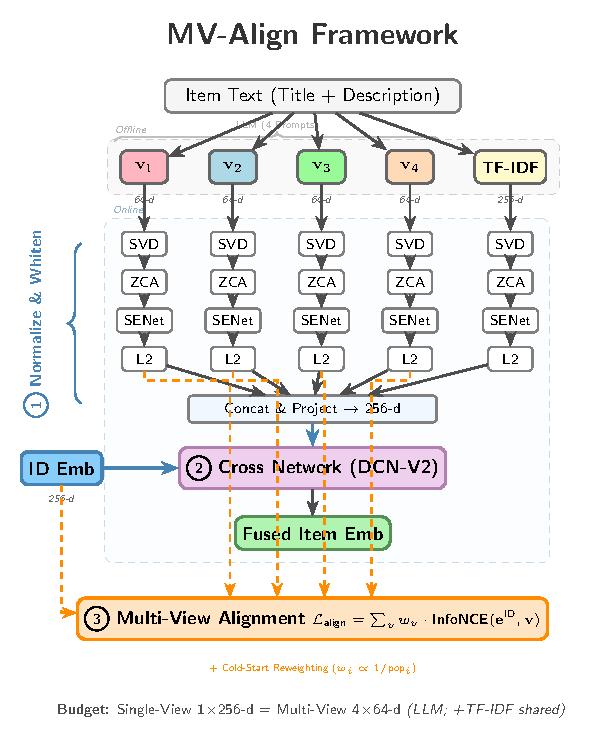
\includegraphics[width=\linewidth]{figures/framework.pdf}%
}{%
  \fbox{\parbox[c][0.22\textheight][c]{0.95\linewidth}{\centering
  \textbf{Framework figure placeholder.}\\
  Put `framework.pdf` under `paper_sigir/figures/`.}}%
}
\caption{Overview of \model.
\circled{1}~\textbf{Prepare}: per-view normalization and whitening (\S\ref{sec:whiten});
\circled{2}~\textbf{Interact}: explicit ID$\times$Text cross via DCN-V2 (\S\ref{sec:cross});
\circled{3}~\textbf{Align}: multi-view contrastive alignment with cold-start reweighting (\S\ref{sec:align}).}
\label{fig:framework}
\end{figure}

\subsection{Training Objective}
We optimize:
\begin{equation}
  \mathcal{L} = \mathcal{L}_{\text{rec}} + \lambda \cdot \mathcal{L}_{\text{mv-align}},
\end{equation}
where $\mathcal{L}_{\text{rec}}$ is the standard sequential
recommendation loss (cross-entropy with sampled negatives), and
$\lambda$ is the alignment weight. Negative sampling is used only
for training efficiency; all evaluation metrics are computed under
full ranking over the entire item set.

\subsection{Model Complexity}\label{sec:complexity}
\textbf{Offline.} \tfidf and \llm item embeddings are precomputed once
and stored as static buffers; SVD reduction and ZCA whitening are computed
offline on the training set.
Each \llm view requires a separate encoder forward pass per item, so
offline encoding cost scales roughly with the number of views (e.g.,
four prompt views vs.\ one for single-view); this is a one-time
(or periodic refresh) cost, amortized over training and serving, and
does not add per-request latency.
\textbf{Online.} The live path adds per-view projections, one DCN-V2
cross layer ($2d{\times}2d$), and fusion MLPs.
Table~\ref{tab:params} reports trainable parameters and framework-estimated
single-forward FLOPs on Amazon Beauty: text fusion and multi-view heads
add modest trainable overhead (${\sim}1.8$M parameters vs.\ \base) while
most parameters remain in the backbone and item embeddings; forward FLOPs
increase by only ${\sim}3\%$ from ID-only to multi-view.
The majority of parameters (${\sim}66$M) reside in the item embedding
table ($|I|{\times}d$); the remaining ${\sim}1$--$3$M cover Transformer
layers, text projections, and cross modules.

\subsection{Two-Phase Training Protocol}
Joint end-to-end training from scratch risks the text heads
overfitting before the backbone converges, because the randomly
initialized projections receive much larger gradients than the
pre-existing ID embeddings. We therefore adopt a two-phase schedule:
\textbf{Phase-A} (warmup) freezes the backbone and trains
text heads and cross modules with a higher learning rate,
grid-searching $(\lambda,\tau)$ on validation;
\textbf{Phase-B} (joint finetune) unfreezes all parameters
with grouped learning rates.
Both modalities are initialized together from epoch~0 so that
text heads receive learning signals while ID embeddings remain
adaptable to text-augmented representations.
Full schedule details are given in \S\ref{sec:experiments}.

\section{Experiments}\label{sec:experiments}
\subsection{Datasets and Evaluation}
We evaluate on two Amazon product review domains~\cite{mcauley2015amazon,ni2019amazon}: \textbf{Beauty} and
\textbf{Toys\&Games}. We follow time-ordered splits and
report metrics under \textbf{full ranking} at $K{=}10$.
In addition to overall metrics (HR, NDCG, MRR, Precision),
we report \textbf{popularity-stratified} metrics by item
interaction counts:
\begin{itemize}[leftmargin=*,itemsep=1pt]
  \item \textbf{new}: $[1,3)$ interactions
  \item \textbf{few}: $[3,10)$ interactions
  \item \textbf{frequent}: $[10,\infty)$ interactions
\end{itemize}
Table~\ref{tab:dataset} summarizes the dataset statistics.
We compute popularity strata from item interaction counts in
the training data.

\begin{table}[h]
\caption{Dataset statistics after 5-core filtering.}
\label{tab:dataset}
\centering
\small
\begin{tabular}{lrrrc}
\toprule
\textbf{Dataset} & \textbf{\#Users} & \textbf{\#Items} & \textbf{\#Inter.} & \textbf{Density} \\
\midrule
Beauty      & 1,210,272 & 259,217 & 2,023,071 & 0.0006\% \\
Toys\&Games & 1,342,912 & 336,080 & 2,252,772 & 0.0005\% \\
\bottomrule
\end{tabular}
\end{table}

\textbf{Main tables} (Table~\ref{tab:main}) report overall metrics and the
\textbf{new} stratum, which is most informative for cold-start;
\textbf{few} and \textbf{frequent} subtables are omitted for brevity
and included in the released artifact.
We report only full-ranking metrics in the
main paper, following prior findings that sampled evaluation
can mis-rank recommender models~\cite{krichene2020sampledmetrics}. Our evaluation
follows leave-one-out next-item prediction with a single
ground-truth item per test case, under which HR@K, Hit@K, and
Recall@K coincide; we use HR@K for brevity and rely on
MRR/NDCG to capture top-position quality.

\subsection{Baselines}
Our comparison design deliberately isolates the contribution of each
text-feature component under a shared backbone (\base), so that
observed gains are attributable to the text augmentation pipeline
rather than confounded by architectural differences across models.
We compare four progressively enriched configurations:
\begin{itemize}[leftmargin=*,itemsep=2pt]
  \item \textbf{\base (ID-only).} Pure sequential baseline
    without text/cross/align.
  \item \textbf{\base + \tfidf.} A lightweight text baseline
    using precomputed \tfidf embeddings with explicit cross
    and alignment.
  \item \textbf{\base + \tfidf + \llm (single-view).} Adds a
    single \llm embedding (Qwen2.5-7B~\cite{qwen2024qwen25}) concatenated with
    \tfidf, using SE-style gating and alignment.
  \item \textbf{\model (multi-view).} \tfidf base view + 4
    multi-view \llm prompt embeddings
    (identity/function/audience/category) with per-view SE-style blocks,
    explicit cross, and multi-view contrastive alignment.
\end{itemize}
\noindent This layered design answers a specific question that
cross-architecture comparisons cannot: \emph{when is each additional
text component worth its cost?} The ablation study
(\S\ref{sec:analysis}) further removes individual modules
(whitening, SE, cross, alignment) to quantify their marginal effects.

\subsection{Implementation Details}
Unless stated otherwise, we use embedding size $d=256$, max
sequence length $L=50$, 2 Transformer layers with 2 heads,
batch size 512, and Adam with base learning rate $10^{-4}$.
\paragraph{Two-phase schedule.}
We follow Phase-A ($15$ epochs) $\rightarrow$ Phase-B ($50$
epochs) with Phase-A selecting $(\lambda,\tau)$ on
$\mathrm{MRR@10}$ for both Beauty and Toys\&Games.
We use grouped learning rates:
$\text{lr}_{\text{text}}=\num{1e-3}$ for text heads,
$\text{lr}_{\text{cross}}=\num{5e-4}$ for cross/DNN blocks,
and $\text{lr}_{\text{backbone}}=\text{lr}_{\text{text}}\times
0.1$ in Phase-B.
\paragraph{Grid.}
For the main runs, we use the Balanced (default) configuration:
$\lambda=0.10$, $\tau=0.05$, training reweighting coefficient
$\beta=3.0$ (Eq.~\eqref{eq:cold_reweight}), and inference boost
$\beta_{\text{infer}}=0.6$ (Eq.~\eqref{eq:infer_boost}) on both datasets
(sensitivity in \S\ref{sec:analysis}).
\paragraph{Training and evaluation protocol.}
We run each configuration with 4 random seeds
$\{42, 2024, 2025, 2026\}$ and report mean$\pm$std;
full-ranking metrics are evaluated at $K{=}10$
with popularity stratification thresholds
\textbf{new}: $[1,3)$, \textbf{few}: $[3,10)$,
\textbf{frequent}: $[10,\infty)$. Our implementation is based on
RecBole~\cite{zhao2021recbole}; all exact settings are
reproducible from the provided configuration files and run scripts
bundled with the artifact.
The released files use the same numerical values as the notation in this paper
(e.g., $\lambda$, $\tau$, $\beta$, and $\beta_{\text{infer}}$ in
\S\ref{sec:experiments} and Eqs.~\eqref{eq:cold_reweight}--\eqref{eq:infer_boost}).
\paragraph{Prompt templates.}
For single-view \llm embeddings we use \texttt{[TITLE] \{text\}} and
extract mean-pooled hidden states from Qwen2.5-7B.
For multi-view embeddings we design four prompts:
(1)~\emph{Identity}: \texttt{Identify the item: [TITLE] \{text\}};
(2)~\emph{Function}: \texttt{What are the main functions and features of [TITLE] \{text\}?};
(3)~\emph{Audience}: \texttt{Who is the target audience or user group for [TITLE] \{text\}?};
(4)~\emph{Category}: \texttt{Categorize the item [TITLE] \{text\} and describe its context.}
Each view is independently encoded, reduced to $d_v{=}64$ via SVD,
and processed through per-view SE-style gating before fusion.

\paragraph{Parameter counts.}
Table~\ref{tab:params} lists trainable parameters and single-forward
FLOPs (framework-estimated) on Amazon Beauty ($|I|{=}259{,}217$,
$d{=}256$, $d_t{=}256$, $d_l{=}1024$, $V{=}4$, $d_v{=}64$).
Multi-view adds ${\sim}1.8$M trainable parameters over ID-only; \llm
embeddings are offline buffers and are not counted as trainable
parameters.

\begin{table}[h]
\caption{Trainable parameters and forward-pass FLOPs (Amazon Beauty).}
\label{tab:params}
\centering
\small
\begin{tabular}{lrrr}
\toprule
\textbf{Model} & \textbf{\#Params} & \textbf{$\Delta$ vs.\ ID} & \textbf{FLOPs} \\
\midrule
\base (ID-only) & 67.2M & --- & 39.5M \\
\base + \tfidf & 68.1M & +0.9M & 39.9M \\
\base + \tfidf + \llm & 68.8M & +1.6M & 40.0M \\
\model (multi-view) & 68.9M & +1.8M & 40.7M \\
\bottomrule
\end{tabular}
\end{table}

\section{Main Results}\label{sec:main_results}
Table~\ref{tab:main} reports full-ranking results on Beauty
and Toys\&Games. Across both datasets, adding text features
consistently improves over the ID-only baseline, with \tfidf
providing substantial gains (+2.6\% HR@10 on Beauty, +6.3\%
on Toys). The key findings are:

\paragraph{Text features provide large gains over ID-only.}
On Beauty, \tfidf alone improves HR@10 from 5.42\% to 5.56\%
(+2.6\%), and NDCG@10 from 2.93\% to 3.69\% (+25.9\%). On
Toys, \tfidf improves HR@10 from 5.92\% to 6.29\% (+6.3\%)
and NDCG@10 from 3.30\% to 4.26\% (+29.1\%).


\paragraph{Multi-view shows consistent improvements.}
\model (7B) achieves the best performance on both datasets.
On \textbf{Beauty}, \model achieves HR@10=5.79\% (+6.8\% vs
ID-only), with MRR@10=3.19\% and NDCG@10=3.80\%. On
\textbf{Toys}, \model achieves HR@10=6.61\% (+11.7\% vs
ID-only), NDCG@10=4.39\%, MRR@10=3.71\%. The hierarchy
\model $>$ TF-IDF+LLM $>$ TF-IDF $>$ ID-only holds for all
overall metrics on both datasets.

\paragraph{Cold-start (new) improvements.}
For the \textbf{new} stratum, \model improves substantially
over text baselines (\tfidf: 1.63\%/1.83\%, single-view \llm:
1.64\%/1.89\%) and narrows the gap to ID-only on Beauty
(1.76\% vs.\ 1.88\%), while exceeding it on Toys (2.04\%
vs.\ 1.92\%). Notably, \model achieves the best NDCG\_new@10
and MRR\_new@10 on both datasets, suggesting that the richer
multi-view text signals primarily improve ranking quality on
cold-start items, while recall coverage remains sensitive to
the fusion configuration.


\begin{table*}[t]
\caption{Main results under full ranking (mean$\pm$std over 4 seeds). Best results per dataset in \textbf{bold}. $^{*}$~$p{<}0.05$, $^{**}$~$p{<}0.01$; paired $t$-test on per-user metric differences against the strongest baseline (Beauty: 146{,}995 test users; Toys: 164{,}590 test users). All values are percentages (\%).}
\label{tab:main}
\centering
\small
\begin{tabular}{lcccccc}
\toprule
\multirow{2}{*}{\textbf{Model}} &
\multicolumn{3}{c}{\textbf{Overall}} &
\multicolumn{3}{c}{\textbf{new stratum} $[1,3)$} \\
\cmidrule(lr){2-4}\cmidrule(lr){5-7}
& HR@10 & NDCG@10 & MRR@10 & HR@10 & NDCG@10 & MRR@10 \\
\midrule
\multicolumn{7}{l}{\textbf{Amazon Beauty}} \\
\base (ID-only, 50ep) & 5.42$\pm$0.21 & 2.93$\pm$0.05 & 2.14$\pm$0.01 & 1.88$\pm$0.03 & 1.05$\pm$0.02 & 0.78$\pm$0.02 \\
\base + \tfidf & 5.56$\pm$0.03 & 3.69$\pm$0.02 & 3.11$\pm$0.01 & 1.63$\pm$0.02 & 1.21$\pm$0.03 & 1.08$\pm$0.03 \\
\base + \tfidf + \llm (7B) & 5.62$\pm$0.03 & 3.73$\pm$0.02 & 3.15$\pm$0.01 & 1.64$\pm$0.03 & 1.24$\pm$0.02 & 1.11$\pm$0.02 \\
\model (7B) & \textbf{5.79}$^{**}$$\pm$0.04 & \textbf{3.80}$^{**}$$\pm$0.02 & \textbf{3.19}$^{*}$$\pm$0.02 & \textbf{1.76}$\pm$0.05 & \textbf{1.28}$\pm$0.02 & \textbf{1.12}$\pm$0.03 \\
\midrule
\multicolumn{7}{l}{\textbf{Amazon Toys\&Games}} \\
\base (ID-only, 50ep) & 5.92$\pm$0.03 & 3.30$\pm$0.02 & 2.48$\pm$0.02 & 1.92$\pm$0.03 & 1.08$\pm$0.02 & 0.81$\pm$0.02 \\
\base + \tfidf & 6.29$\pm$0.03 & 4.26$\pm$0.01 & 3.64$\pm$0.01 & 1.83$\pm$0.03 & 1.38$\pm$0.02 & 1.23$\pm$0.02 \\
\base + \tfidf + \llm (7B) & 6.39$\pm$0.02 & 4.32$\pm$0.01 & 3.67$\pm$0.01 & 1.89$\pm$0.05 & 1.41$\pm$0.03 & 1.26$\pm$0.02 \\
\model (7B) & \textbf{6.61}$^{**}$$\pm$0.03 & \textbf{4.39}$^{**}$$\pm$0.03 & \textbf{3.71}$^{*}$$\pm$0.02 & \textbf{2.04}$\pm$0.03 & \textbf{1.47}$\pm$0.02 & \textbf{1.29}$\pm$0.02 \\
\bottomrule
\end{tabular}
\end{table*}

\section{Analysis}\label{sec:analysis}

We conduct systematic ablation studies to answer RQ1--RQ4.
All ablations use multi-view 7B on Toys\&Games; relative changes
are derived from controlled experiments.
\subsection{Component Ablation (RQ1--RQ4)}

Table~\ref{tab:ablation} groups ablations by research question on
Toys\&Games (7B): whitening (RQ1), SE-style gating and explicit cross
(RQ2; cross also addresses RQ4), contrastive alignment (RQ4).
For \textbf{RQ3} (multi-view vs.\ single-view under equal bandwidth),
compare \emph{Multi-view w/ Whiten} vs.\ \emph{Single-view w/ Whiten}
within the RQ1 block.

\begin{table}[t]
\caption{Component ablation on Toys\&Games (7B), ordered by RQ1$\rightarrow$RQ2$\rightarrow$RQ4.
RQ3 is read by comparing the two whitening rows marked for multi-view vs.\ single-view.
The Full row (HR@10=6.58) differs slightly from Table~\ref{tab:main} (6.61) because ablations use a single representative seed rather than the 4-seed mean.
All values in \%.}
\label{tab:ablation}
\centering
\scriptsize
\begin{tabular}{@{}lcccc@{}}
\toprule
\textbf{Configuration} & HR@10 & NDCG@10 & MRR@10 & HR\_new@10 \\
\midrule
\multicolumn{5}{l}{\textit{RQ1 (whitening)}} \\
Multi-view w/ Whiten & 6.58 & 4.40 & 3.72 & 2.07 \\
Multi-view w/o Whiten & 6.46 & 4.34 & 3.68 & 1.97 \\
Single-view w/ Whiten & 6.41 & 4.33 & 3.68 & 1.94 \\
Single-view w/o Whiten & 6.36 & 4.29 & 3.65 & 1.89 \\
\midrule
\multicolumn{5}{l}{\textit{RQ2 (SE-style); RQ4 (explicit cross)}} \\
Full (SE + Cross) & 6.58 & 4.40 & 3.72 & 2.07 \\
$-$ SE-style & 6.62 & 4.39 & 3.70 & 2.00 \\
$-$ Cross & 7.22 & 4.23 & 3.31 & 2.73 \\
$-$ SE $-$ Cross & 7.23 & 4.24 & 3.31 & 2.70 \\
\midrule
\multicolumn{5}{l}{\textit{RQ4 (contrastive alignment)}} \\
$-$ Align & 6.41 & 4.35 & 3.71 & 1.83 \\
\bottomrule
\end{tabular}
\end{table}

\paragraph{Whitening benefits multi-view but not single-view (RQ1).}
For multi-view, removing whitening reduces HR@10, revealing
that whitening primarily benefits recall coverage by decorrelating
multi-view features. For single-view (TF-IDF+LLM), removing
whitening has minimal impact, confirming that single-view LLM
features are already well-conditioned.

\paragraph{SE-style gating has minor impact (RQ2).}
Removing SE-style gating alone causes only marginal changes on
most metrics. This is expected: per-view whitening already
decorrelates feature dimensions and $\ell_2$ normalization
equalizes view magnitudes, leaving little residual scale
mismatch for channel gating to correct.
The combination of removing both SE and Cross shows the largest
HR\_new@10 gains, indicating that these components together
calibrate toward frequent items.

\paragraph{Cross Network is essential for ranking quality (RQ4).}
Removing the cross module increases HR@10 but \emph{sharply degrades}
ranking metrics (MRR@10 and NDCG@10).
This reveals a fundamental \textbf{HR--ranking trade-off}: without
explicit cross interactions, the model produces smoother score
distributions that improve coverage but lose discriminative power
for top-1 ranking.

\paragraph{Contrastive alignment helps overall and cold-start recall (RQ4).}
Disabling the multi-view InfoNCE alignment objective lowers HR@10
from 6.58\% to 6.41\% and HR\_new@10 from 2.07\% to 1.83\%, with
small drops in NDCG@10 and MRR@10 (4.40\%$\rightarrow$4.35\%,
3.72\%$\rightarrow$3.71\%).
Unlike the cross ablation, this is not an HR--ranking inversion:
alignment uniformly strengthens text--ID coupling and is most
visible on the \textbf{new} stratum.

\subsection{RQ3: Multi-view vs.\ Single-view Under Equal Bandwidth}

We compare single-view TF-IDF+LLM (256-d LLM embedding) against
multi-view \model ($4\times 64$-d = 256-d total LLM budget) using
Table~\ref{tab:main}; the RQ1 whitening rows in Table~\ref{tab:ablation}
isolate the same comparison under controlled ablations on Toys\&Games.

\paragraph{Takeaway.}
Under equal embedding bandwidth, multi-view outperforms
single-view on all metrics on both datasets, with gains most
pronounced on the \textbf{new} stratum (cf.\ the cold-start
analysis in \S\ref{sec:main_results}). Diverse prompt perspectives
particularly help low-popularity items.

\subsection{Understanding the HR--Ranking Trade-off}

\begin{figure}[t]
\centering
\begin{subfigure}[t]{0.48\linewidth}
  \centering
  \IfFileExists{figures/tradeoff_mrr.pdf}{%
    
\includegraphics[width=\linewidth]{figures/tradeoff_mrr.pdf}%
  }{%
    \fbox{\parbox[c][0.15\textheight][c]{0.9\linewidth}{\centering
    \textbf{HR--MRR Trade-off}\\
    Run \texttt{plot\_tradeoff.py}}}%
  }
  \caption{HR@10 vs.\ MRR@10}
  \label{fig:tradeoff_mrr}
\end{subfigure}
\hfill
\begin{subfigure}[t]{0.48\linewidth}
  \centering
  \IfFileExists{figures/tradeoff_ndcg.pdf}{%
    
\includegraphics[width=\linewidth]{figures/tradeoff_ndcg.pdf}%
  }{%
    \fbox{\parbox[c][0.15\textheight][c]{0.9\linewidth}{\centering
    \textbf{HR--NDCG Trade-off}\\
    Run \texttt{plot\_tradeoff.py}}}%
  }
  \caption{HR@10 vs.\ NDCG@10}
  \label{fig:tradeoff_ndcg}
\end{subfigure}
\caption{HR--ranking trade-off on Toys\&Games (7B). Points follow
Table~\ref{tab:ablation} (RQ1--RQ4). The dashed arrow
contrasts Full vs.\ $-$Cross: higher HR@10 (+9.7\%) but lower MRR@10
($-$11.0\%) and NDCG@10 ($-$3.9\%). The $-$Align point lies near Full
but is uniformly lower (\S\ref{sec:analysis}).}
\label{fig:tradeoff}
\end{figure}

We observe a trade-off between HR and ranking metrics (MRR/NDCG) that
may seem counter-intuitive---better ranking quality typically correlates
with higher hit rates. However, under \textbf{full ranking}, this
trade-off emerges naturally.

\paragraph{Mechanism.}
The cross network produces \emph{sharper score distributions}:
a few items receive significantly higher scores, creating a
``winner-take-all'' effect that benefits top-1 accuracy (MRR)
but may push relevant items just outside the top-$K$ cutoff (hurting HR@$K$).
In contrast, removing cross yields \emph{smoother score distributions}:
more items cluster near the decision boundary,
allowing more ground-truth items to enter top-$K$ (higher HR)
at the cost of less precise top-1 ranking (lower MRR).

\paragraph{Empirical evidence.}
Table~\ref{tab:ablation} quantifies this trade-off:
\textbf{removing cross} raises HR@10 from 6.58\% to 7.22\% (+9.7\%)
but drops MRR@10 from 3.72\% to 3.31\% ($-$11.0\%) and NDCG@10
from 4.40\% to 4.23\% ($-$3.9\%).
Conversely, \textbf{enabling cross} sharpens ranking precision
at the cost of recall coverage.
Figure~\ref{fig:tradeoff} visualizes HR vs.\ ranking metrics across
ablation points from Table~\ref{tab:ablation} (including whitening
and $-$Align); the dashed arrow highlights the cross-network
HR--ranking trade-off. The left panel shows HR--MRR; the right
panel shows HR--NDCG.

\paragraph{Practitioner guidance.}
This trade-off maps directly to deployment scenarios:
\begin{itemize}[leftmargin=*,itemsep=2pt]
  \item \textbf{Candidate generation / recall-oriented systems}:
    Disable cross to achieve higher HR at the cost of lower MRR/NDCG.
  \item \textbf{Final ranking / precision-oriented systems}:
    Enable cross to sharpen score distributions and improve MRR/NDCG.
\end{itemize}

\subsection{Hyperparameter Sensitivity}

\begin{figure}[t]
\centering
\IfFileExists{figures/sensitivity_tradeoff_ndcg.pdf}{%
  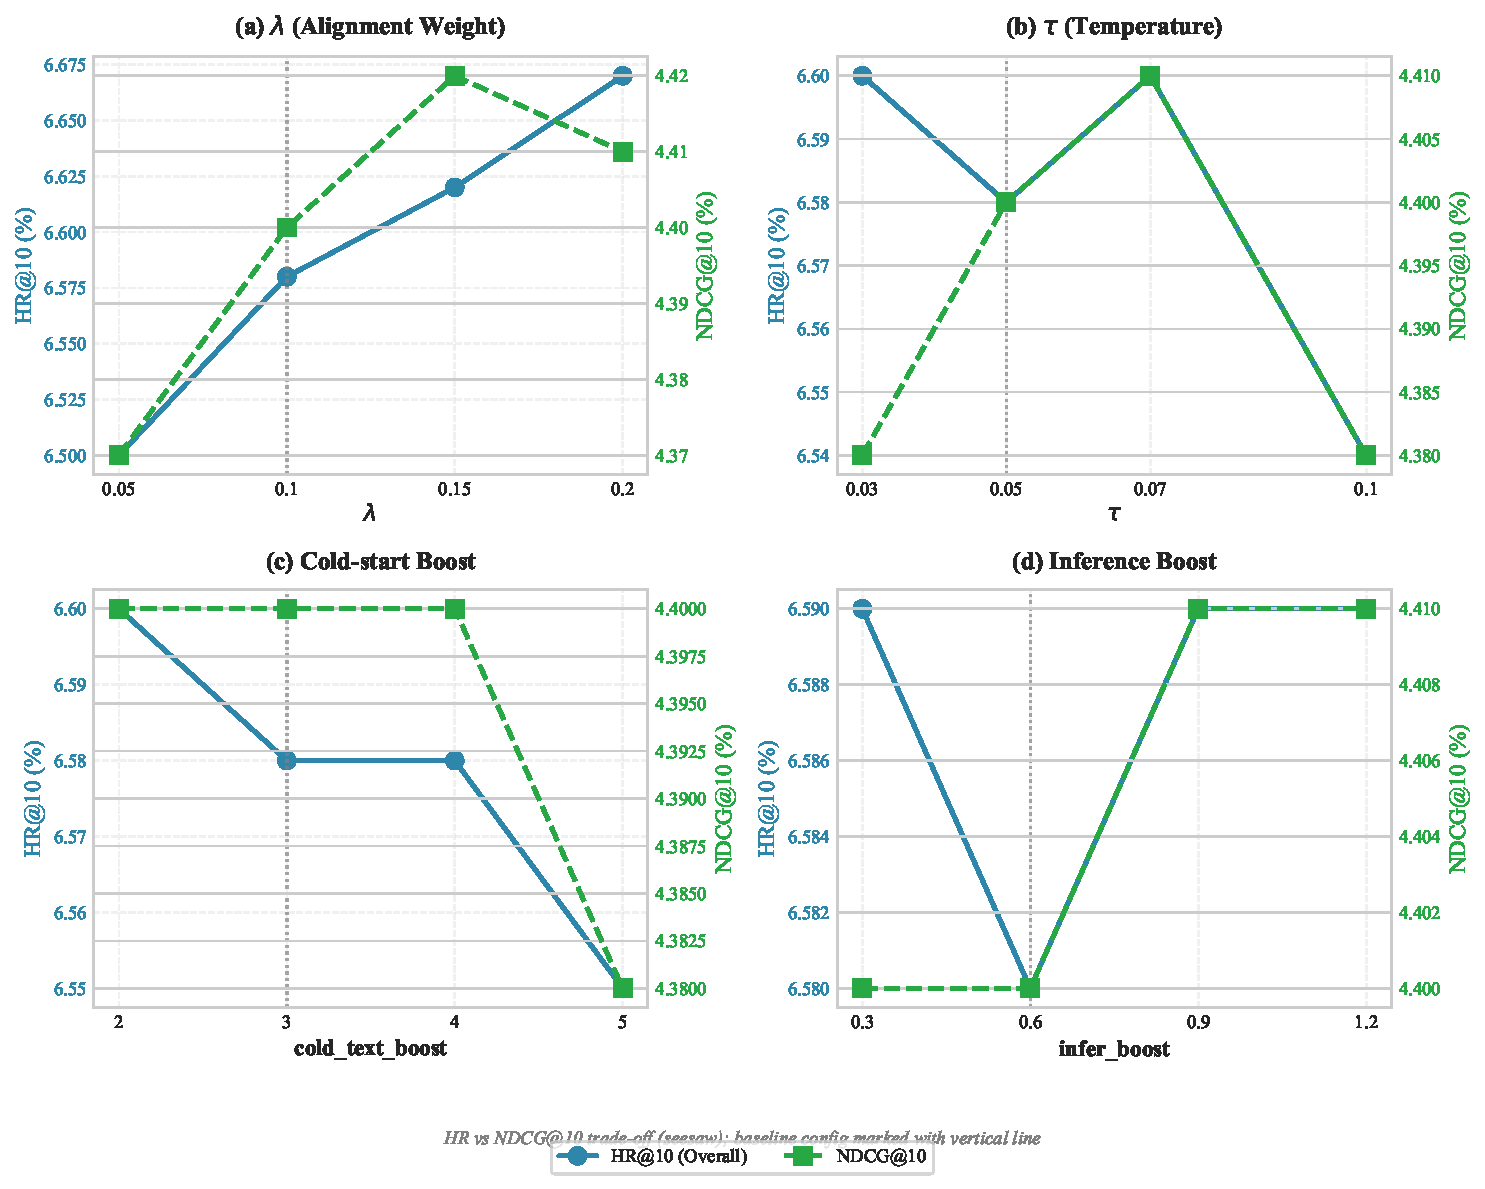
\includegraphics[width=\linewidth]{figures/sensitivity_tradeoff_ndcg.pdf}%
}{%
  \fbox{\parbox[c][0.25\textheight][c]{0.9\linewidth}{\centering
  \textbf{Sensitivity Analysis}\\
  Run \texttt{plot\_sensitivity.py}}}%
}
\caption{Hyperparameter sensitivity on Toys\&Games (7B). Each panel
varies one parameter while holding the others at default values
(dashed vertical line). HR@10 (solid, left axis) and NDCG@10
(dashed, right axis) remain stable across these settings, with
total variation under 0.2 pp for HR@10 and under 0.05 pp for
NDCG@10.}
\label{fig:sensitivity}
\end{figure}

Figure~\ref{fig:sensitivity} shows the sensitivity of \model to
$\lambda$, $\tau$, $\beta$ (Eq.~\eqref{eq:cold_reweight}), and
$\beta_{\text{infer}}$ (Eq.~\eqref{eq:infer_boost}) on Toys\&Games (7B),
plotting HR@10 (left axis) and NDCG@10 (right axis) as each varies
while the others are held at their default values ($\lambda{=}0.10$,
$\tau{=}0.05$, $\beta{=}3.0$, $\beta_{\text{infer}}{=}0.6$).

\paragraph{Alignment weight $\lambda$ and temperature $\tau$.}
Both contrastive hyperparameters show smooth, unimodal curves.
HR@10 ranges from 6.50\% ($\lambda{=}0.05$) to 6.67\%
($\lambda{=}0.20$), a spread of only 0.17 pp; NDCG@10 peaks at
$\lambda{=}0.15$ (4.42\%) and remains within 0.05 pp across the
grid. Temperature $\tau$ is similarly stable: HR@10 varies by
0.06 pp and NDCG@10 by 0.03 pp over the tested range
($0.03$--$0.10$). This confirms that the contrastive objective is
robust to moderate tuning.

\paragraph{Cold-start boost and inference boost.}
The training coefficient $\beta$ (Eq.~\eqref{eq:cold_reweight}) has minimal impact on overall
metrics (HR@10 within 0.05 pp, NDCG@10 within 0.02 pp), as it
primarily affects the training-time reweighting of low-popularity
items. The inference coefficient $\beta_{\text{infer}}$ is similarly stable for overall
performance (HR@10 within 0.01 pp). Consistent with
Eq.~\eqref{eq:infer_boost}, it modulates text reliance for
low-popularity items at inference time; overall HR@10 and
NDCG@10 remain within the narrow bands above across the tested grid.

\paragraph{Takeaway.}
These hyperparameters exhibit low sensitivity on overall metrics,
with total variation under 0.2 pp for HR@10 and under 0.05 pp for
NDCG@10. This makes \model easy to tune in practice: the default
configuration performs near-optimally, and practitioners can adjust
$\lambda$ or $\beta_{\text{infer}}$ to trade off between overall and
cold-start performance without risking large regressions.

\section{Conclusion}
We presented \model, a method that brings explicit cross networks and
multi-view \llm text alignment to sequential recommendation.
Full-ranking experiments on Amazon Beauty and Toys\&Games yield three
actionable takeaways:

\textbf{(1) TF-IDF is a surprisingly strong baseline.}
\tfidf alone provides substantial gains over ID-only baselines
(+2.6\%/+6.3\% HR@10 on Beauty/Toys) and should be the
\emph{first} text enhancement before investing in \llm embeddings.

\textbf{(2) Multi-view improves cold-start ranking under equal bandwidth.}
Under equal embedding bandwidth ($4{\times}64$-d vs.\ $1{\times}256$-d),
multi-view \llm prompting yields the best cold-start ranking quality:
\model achieves the highest NDCG\_new@10 and MRR\_new@10 on both
datasets, while narrowing the HR\_new gap to ID-only on Beauty
(1.76\% vs.\ 1.88\%) and exceeding it on Toys
(2.04\% vs.\ 1.92\%).

\textbf{(3) The cross network governs the HR--MRR/NDCG trade-off.}
Enabling cross sharpens ranking quality (MRR/NDCG) at the cost of
recall (HR); disabling it reverses this balance. This maps directly
to deployment scenarios: disable cross for candidate generation,
enable it for final re-ranking.

\smallskip\noindent
All code and configuration files are available at
\texttt{\url{https://anonymous.4open.science/r/recbole-multiview-D83A}}.

\bibliographystyle{unsrt}
\bibliography{refs}

%% ====================================================================
%% APPENDIX REMOVED for RecSys Main Track Long submission (8pp + refs).
%% All auxiliary analyses are provided in the anonymous repository:
%%   https://anonymous.4open.science/r/recbole-multiview-D83A
%%
%% Contents moved to repo:
%%   - Sampled evaluation sanity check (uni100 vs. full ranking)
%%   - Hyperparameter configurations (Balanced / Cold-Tail-optimized presets)
%%   - Sensitivity analysis on 4 key hyperparameters
%%   - Seed stability analysis (4 seeds)
%%   - Extended strata results (few / frequent)
%% ====================================================================

\end{document}


